\documentclass[crop,tikz,border=0px,convert=pdf2svg,multi=false]{standalone}
\usepackage{amsfonts}
\usepackage{amsmath}
\usepackage{mathtools}
\usepackage[defaultsans]{opensans}
\usetikzlibrary{shapes,arrows,positioning}
\begin{document}
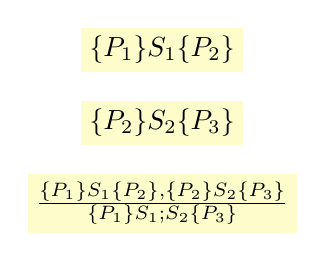
\begin{tikzpicture}[font=\sffamily, node distance=1em,
  every node/.style = {draw=none, fill=yellow!20, align=center, inner
    sep=.3em, text centered}]

  \node (n0) {\(\{P_1\}S_1\{P_2\}\)};
  \node [below=of n0] (n1) {\(\{P_2\}S_2\{P_3\}\)};
  \node [below=of n1] {\(\frac{\{P_1\}S_1\{P_2\},\{P_2\}S_2\{P_3\}}{\{P_1\}S_1;S_2\{P_3\}}\)};

\end{tikzpicture}
\end{document}
